\section{研究背景和动机}
\label{chap:hash:motivation}

本节对该方法中涉及的相关背景进行介绍,包括网络噪声对时间隐通道的干扰方式,以及基于码字间校验的鲁棒性策略。其中,网络噪声对时间隐通道的干扰,主要分析了不同类型的网络噪声对鉴别过程的干扰情况,并提出了解决方案。基于码字间检验的鲁棒性策略,提出了码字间校验关系,提高了校验信息利用率。

\subsection{网络噪声对时间隐通道的干扰}
\label{chap:hash:motivation:noise}

由图\nref{fig:2:pmf-dropout}可知,VoLTE视频通话中长度为1的随机丢包占比在50\%左右,其余的均为连续丢包事件。通过CRC检错码等方式,对离散的随机丢包噪声具有较好的抑制作用。对于连续丢包噪声的干扰,校验过程出现误匹配的概率较高,码字鉴别准确率降低,最终导致误码率升高。

\insertFigure{
	\begin{figure}[htbp]
		\centering
        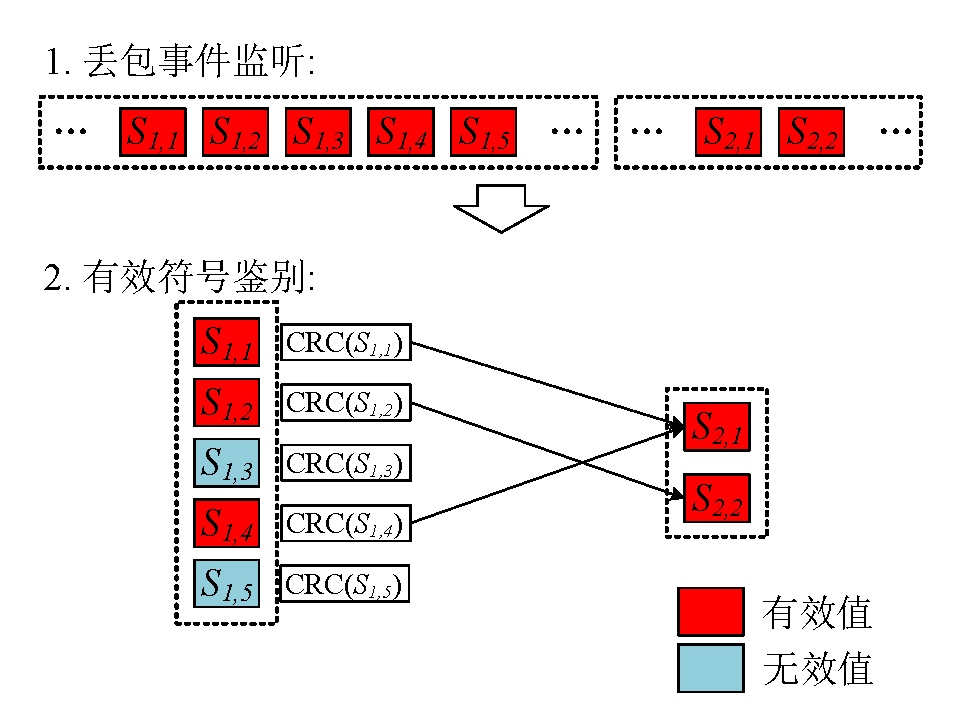
\includegraphics[width=0.7\textwidth]{chapters/chapter5/figures/crc-continuous.pdf}
        \caption{连续丢包对鉴别过程的影响示意图}
        \label{fig:5:crc-continuous}
	\end{figure}
}

如图\nref{fig:5:crc-continuous},存在连读丢包的情况下,校验能力存在明显退化。第一组$S_{1}$为待验证的数据符号,第二组$S_{2}$为可能的校验符号。在有效符号鉴别过程中,依次计算CRC($S_{1,\ i}$),并将结果与$S_{2,\ j}$比较。由于校验符号只是CRC散列结果的一部分,存在碰撞的概率较高。最终的鉴别结果,只能识别出部分网络噪声。由于缺乏额外信息,无法进一步判别噪声,从而出现误码。

理想情况下,按照本文\nref{chap:zigzag:model:modulation:crc}中设计的鲁棒性方案,当数据码字中出现噪声而校验码字中无噪声时,出现误码的概率为$1/L_{Codeword}$,具备有效的鉴别能力。而实际场景中,校验码字也会受噪声干扰,出现图\nref{fig:5:crc-continuous}中鉴别失效的情况。

\insertFigure{
	\begin{figure}[htbp]
		\centering
        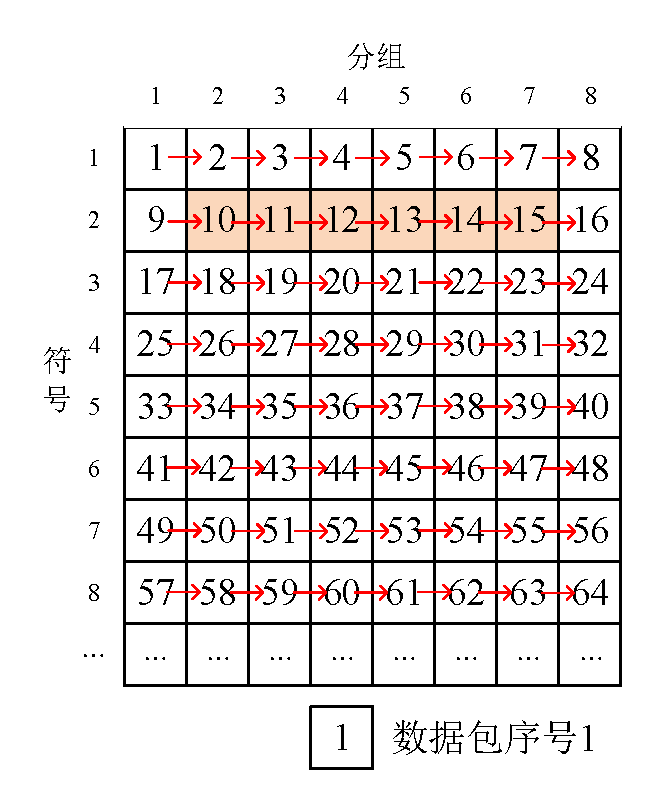
\includegraphics[width=0.45\textwidth]{chapters/chapter5/figures/row-matrix.pdf}
        \caption{符号-数据包序号映射矩阵示意图}
        \label{fig:5:row-matrix}
	\end{figure}
}

VoLTE视频通话中,丢包存在随机性,出现密集连续丢包的概率较低。因此,将连续丢包分散到不同组,利用每组的校验能力降低噪声干扰,是应对该类型噪声的可行办法。如图\nref{fig:5:row-matrix},矩阵中的元素为数据包序号,矩阵的列号为组号,矩阵的行号对应符号。当出现连续丢包噪声,如$10\sim 15$,经过该映射矩阵处理,噪声被分配到分组$2\sim 7$。该映射矩阵模式,有利于充分利用每组的校验能力,提高校验资源利用率。

\subsection{基于码字间校验的鲁棒性策略}
\label{chap:hash:motivation:robustness}

时间隐通道的鲁棒性策略中,包含喷泉码等无速率编码,通过结合多个码字之间的冗余数据,还原真实的消息内容。\nupcite{6296078}在区块链技术中,每一个区块均含有前一个区块的HASH值,因此当链长达到一定规模时,起始区块得到充分验证。\nupcite{7467408}对于基于主动丢包的时间隐通道,由于噪声分布不均匀,利用低噪声阶段的信息校验高噪声阶段的信息,能够进一步提高校验信息利用率。

\insertFigure{
	\begin{figure}[htbp]
		\centering
        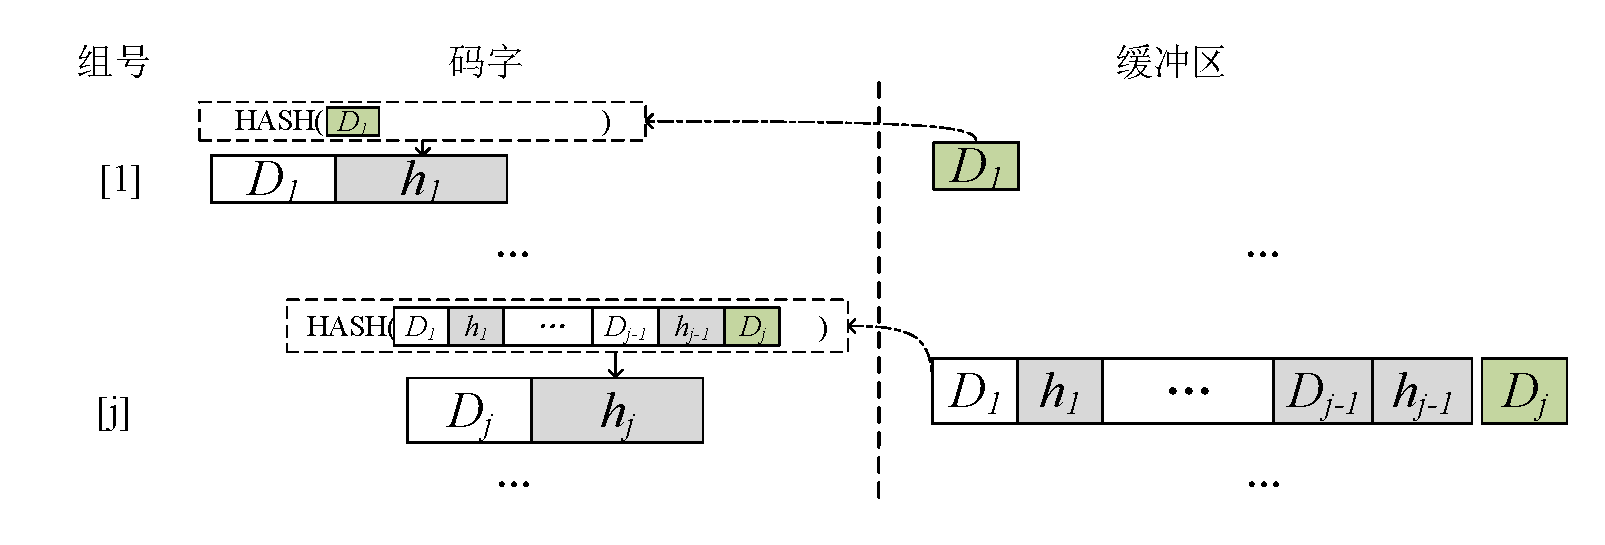
\includegraphics[width=0.95\textwidth]{chapters/chapter5/figures/chain-example.pdf}
        \caption{码字间校验结构示意图}
        \label{fig:5:chain-example}
	\end{figure}
}

如图\nref{fig:5:chain-example},码字间校验块$h_{j}$记录了数据缓冲区的散列值。借助HASH函数的随机性和确定性,随着接收过程推进,通过后接收码字中的码字间校验信息,验证已经接收到码字的正确性。即使部分码字受噪声干扰无法鉴别,借助其它组中的有效信息,实现跨组验证。

HASH摘要在计算时进行了加盐处理,通过结合用户自定义盐值及RTP随机字段,提高了时间隐通道保密性。监听者无法获取盐值,从而无法正确恢复码字间校验块$h_{j}$,码字间校验关系得到保护。存在噪声干扰时,监听者无法区分噪声及信号,隐蔽消息得到保护。

\subsection{研究动机}
\label{chap:hash:motivation:motivation}

本时间隐通道构建方法,基本的调制方式为主动丢包,调制结果隐匿在网络噪声中。通过多重校验的方式有效去噪,提高鲁棒性降低误码率。在多重校验过程中,引入加盐及随机化过程,增加随机性与保密性。

\insertFigure{
	\begin{figure}[htbp]
		\centering
        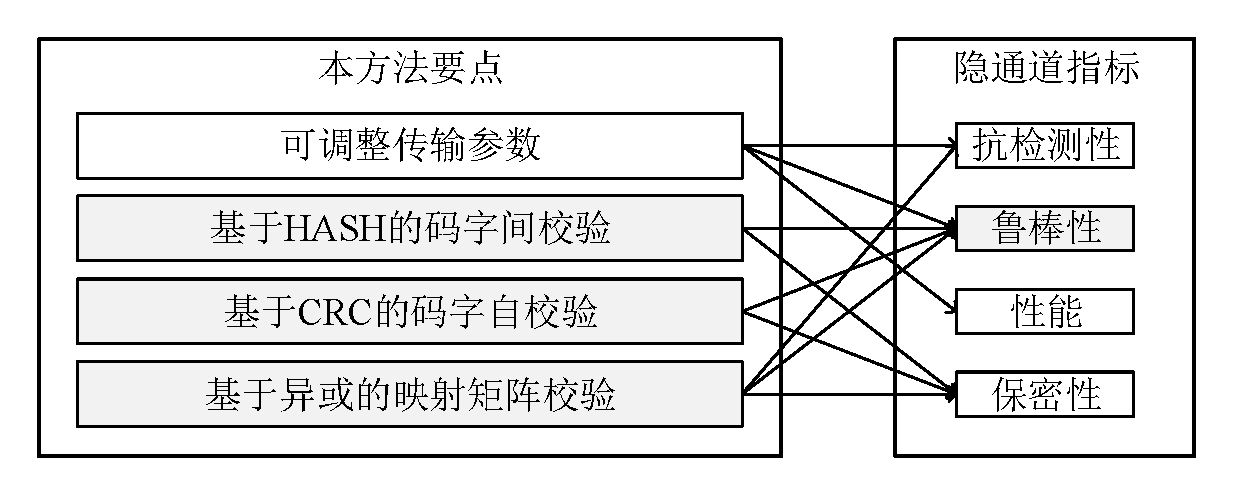
\includegraphics[width=0.8\textwidth]{chapters/chapter5/figures/chapter-struct.pdf}
        \caption{基于多重校验的时间隐通道构建方法研究要点与指标}
        \label{fig:5:chapter-struct}
	\end{figure}
}

如图\nref{fig:5:chapter-struct},本方法的要点主要包括可调整传输参数、基于HASH的码字间校验、基于CRC的码字自校验及基于异或的映射矩阵校验。其中,可调整传输参数主要解决抗检测性、鲁棒性及传输性能之间的均衡问题。该方法需要牺牲性能保证鲁棒性,因此通过调整传输参数实现各方面均衡。基于HASH的码字间校验、基于CRC的码字自校验,主要提升时间隐通道的鲁棒性,同时提高隐蔽消息的保密性。基于异或的映射矩阵校验,通过构建具有校验能力的映射矩阵,在分散丢包事件的基础上提高鲁棒性。